We were mainly interested in answering two questions:

\begin{enumerate}

  \item how far in the future can our system predict well?

  \item how does the knowledge of the grasped object affect the error?

\end{enumerate}

In order to answer the first question, we have checked how the error
on regression changes as the \emph{blind fraction} $0 \leq B \leq 1$
of the grasp increases from $0.1$ to $0.5$. The blind fraction
indicates what percentage of the grasp, from the contact point
backwards, is hidden to the system (Figure \ref{fig:B_example} shows a
typical situation). It was intuitively expected that larger values of
$B$ would smoothly lead to larger errors.

\begin{figure}[htbp]
  \begin{center}
    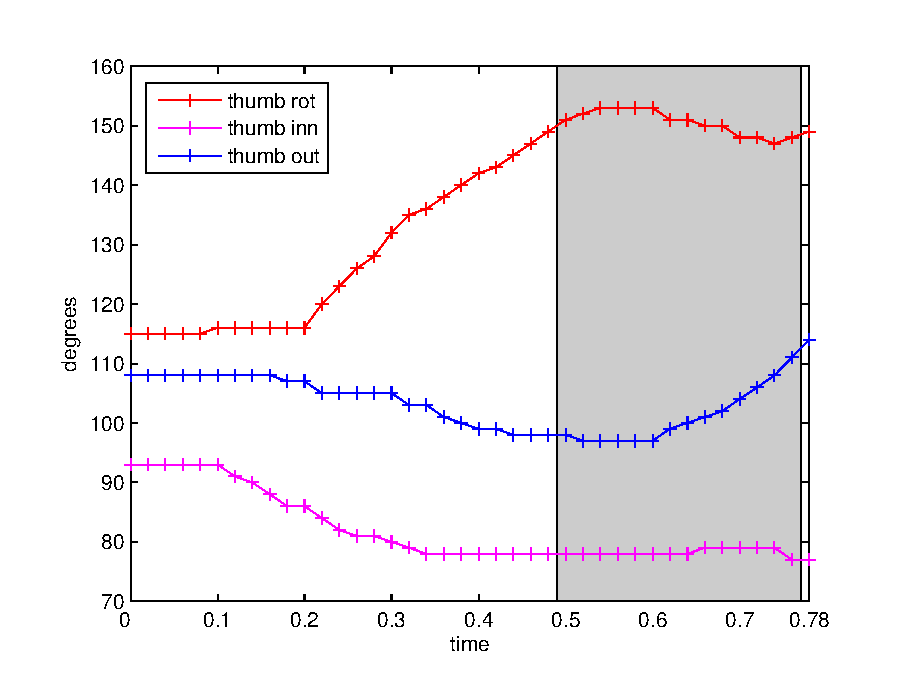
\includegraphics[width=0.5\linewidth]{B_example.eps}
    \caption{The blind window (the grey zone in the Figure) indicates
    what fraction of each grasp, from the contact point backwards, is
    hidden to the SVM. The data shown is a typical trajectory of the
    thumb (rotation, inner phalanx, outer phalanx) during a grasp. In
    this case the grasp lasts $0.78$ seconds and $B=0.375$. The last
    sample (for $t=0.78$) is the target value.}
    \label{fig:B_example}
  \end{center}
\end{figure}

This procedure was repeated independently for each single sensor; the
regression error obtained is the error attained by $2$-fold cross
validation with the optimal $C$ and $\sigma$, determined using the
procedure detailed in the previous Section. The errors for each sensor
were then grouped and averaged accordingly to their measurement unit
and meaning: the position of the hand ($3$ sensors, the $x,y,z$ from
the FoB), the hand orientation ($3$ sensors, the azimuth, elevation
and roll from the FoB), and the posture of the hand ($22$ sensors, the
joint positions from the CyberGlove). According to the device
resolutions (see the previous Section), we set $\epsilon$ to $0.1$
inches for the hand position, $0.5$ degrees for the hand orientation
and $1$ degree for the hand posture.

In order to answer the second question, we first compared the error
obtained as described above using all sessions for each single object,
so to obtain an estimate of how complex it is to approximate the grasp
for the can, roll and mug, unbiased by the differences among the
subjects. Subsequently we averaged these three errors and compared the
average with the overall error, obtained by joining \emph{all}
sessions together in a single training set. Figure \ref{fig:err_all}
shows the experimental results.

\begin{figure}[htbp]
  \begin{center}
    \begin{tabular}{cc}
      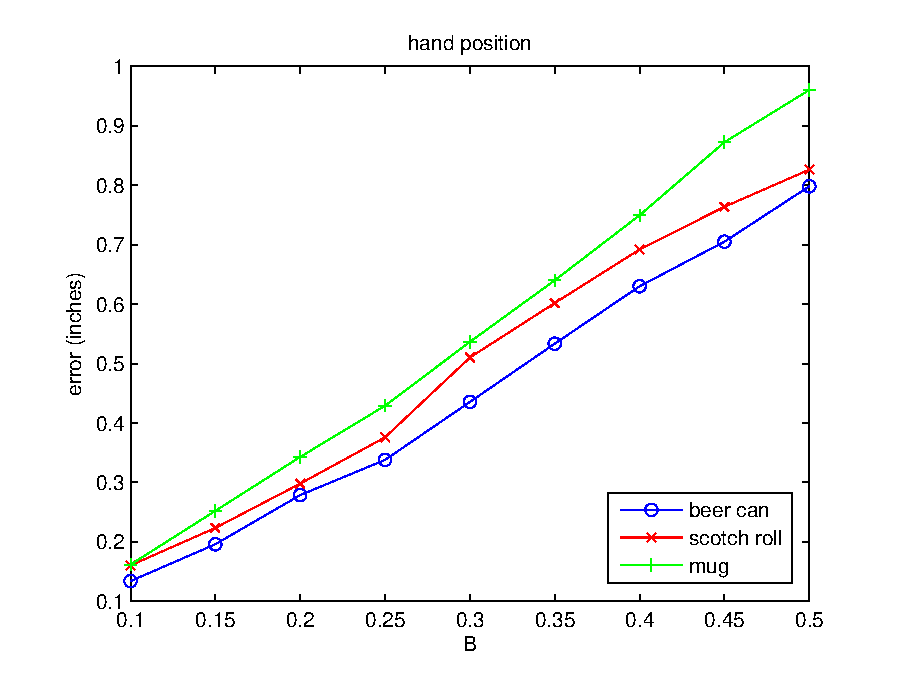
\includegraphics[width=0.45\textwidth]{error_pos.eps} &
      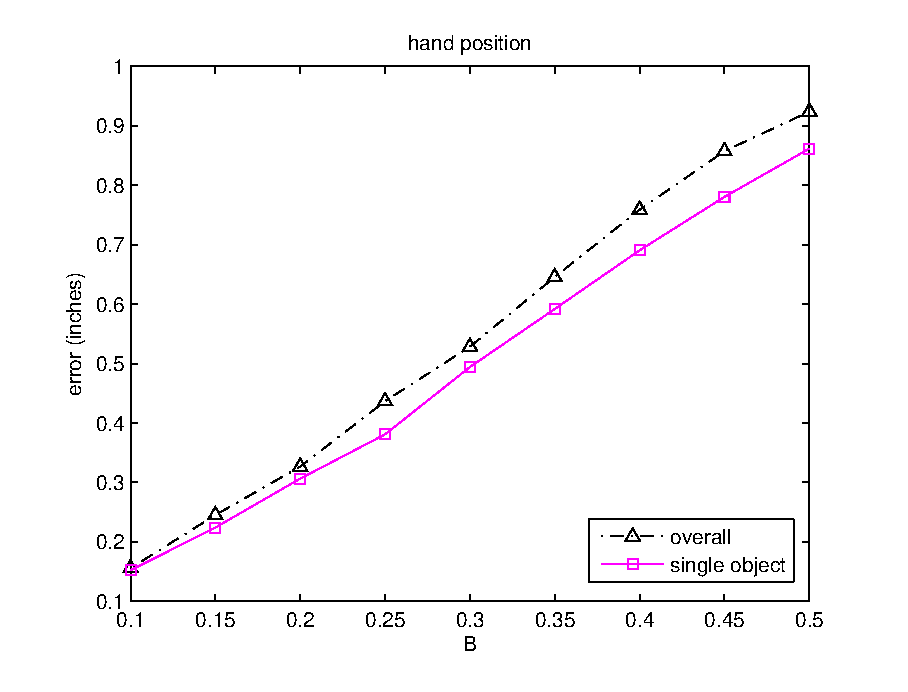
\includegraphics[width=0.45\textwidth]{error_cmp_pos.eps} \\
      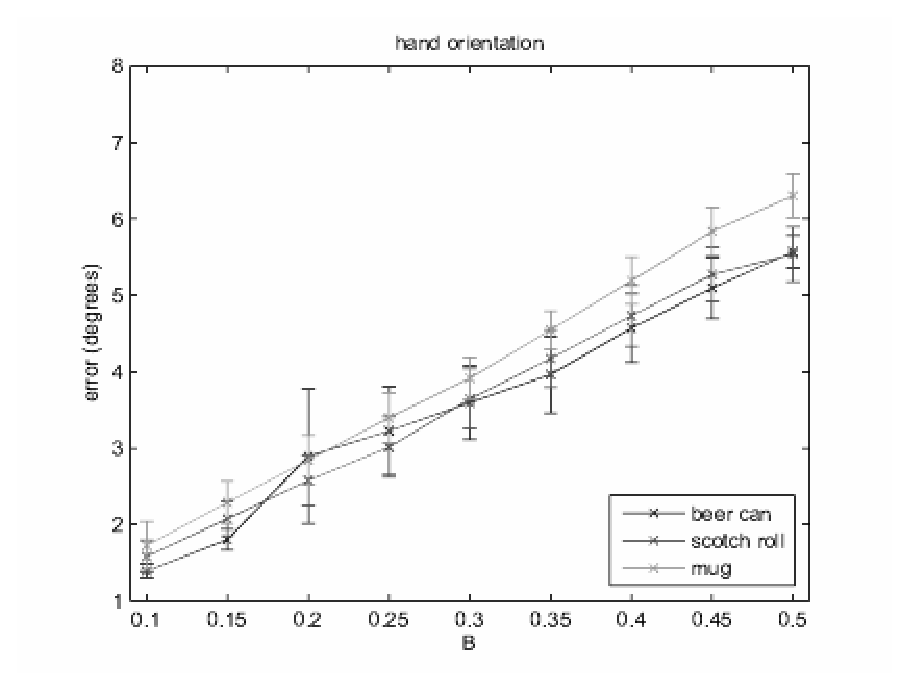
\includegraphics[width=0.45\textwidth]{error_ori.eps} &
      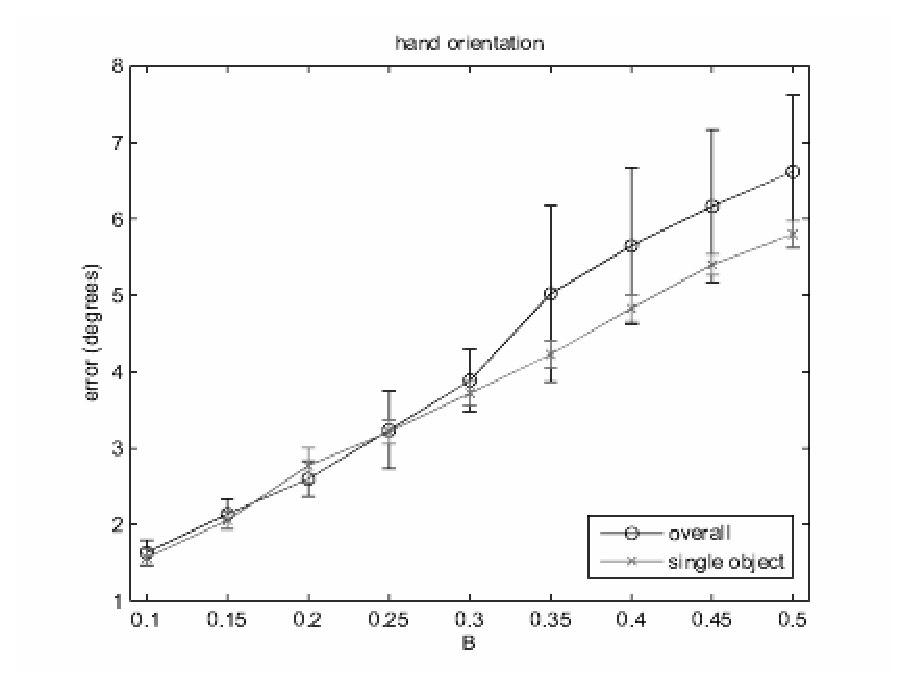
\includegraphics[width=0.45\textwidth]{error_cmp_ori.eps} \\
      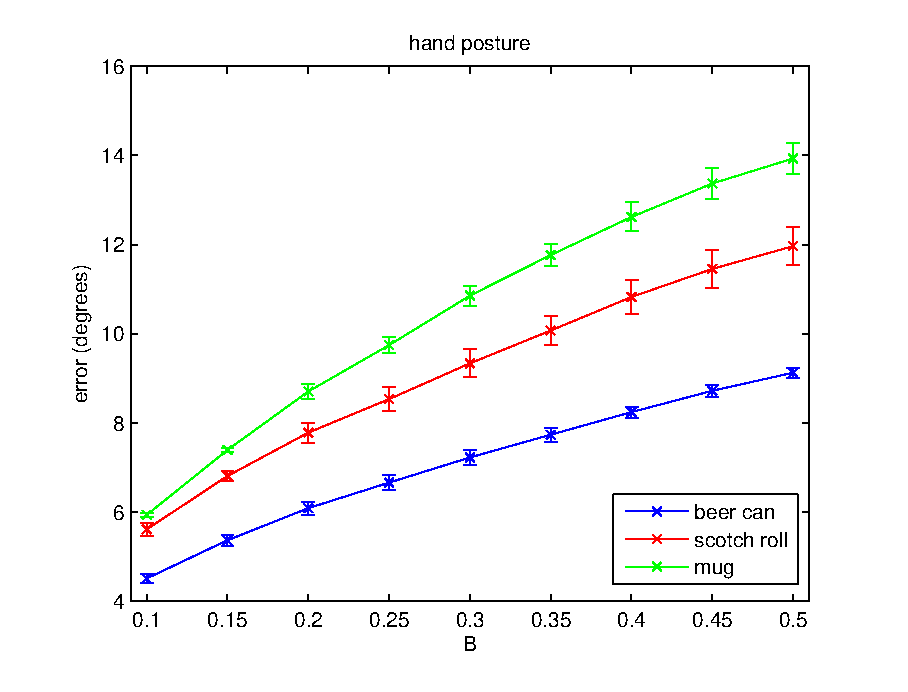
\includegraphics[width=0.45\textwidth]{error_pst.eps} &
      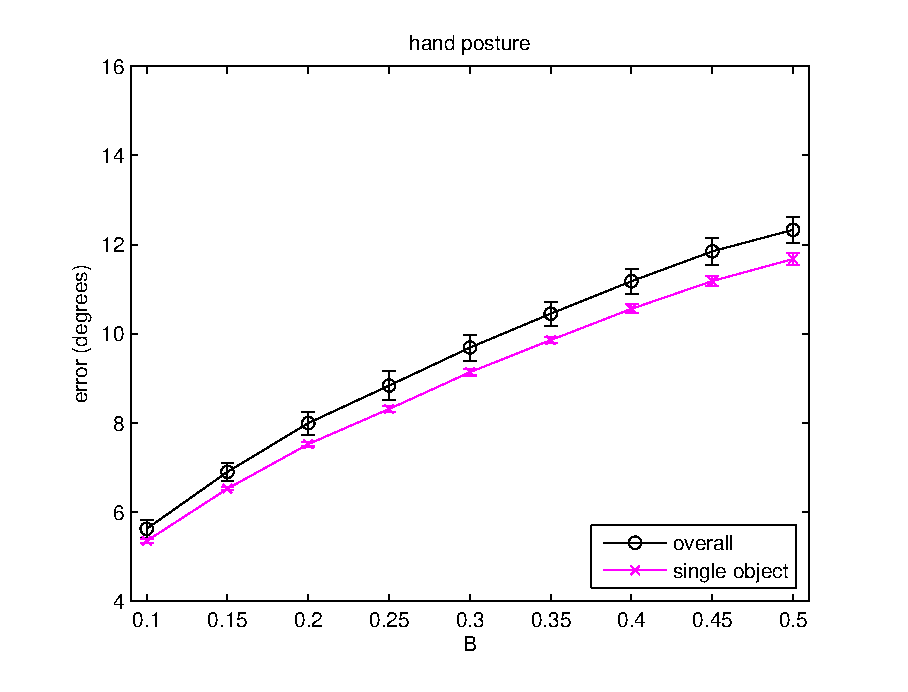
\includegraphics[width=0.45\textwidth]{error_cmp_pst.eps} \\
    \end{tabular}
    \caption{Regression results as the blind fraction $B$ increases
    from $0.1$ to $0.5$. In each row, representing a different set of
    sensors (in turn, hand position, orientation and posture), the
    left-hand side pictures compare the errors on different objects,
    while the right-hand side pictures compare the average error on
    single objects and the overall error.}
    \label{fig:err_all}
  \end{center}
\end{figure}

Consider Figure \ref{fig:err_all}, left column: as one can see, as far
as the hand position and orientation are concerned, the three objects
show a comparable error. On the other hand, there is a precise ranking
in the hand posture regression: the mug is more difficult than the
scotch roll, which is in turn harder than the beer can. This is
intuitively sensible, since it is possible to grasp the scotch roll in
more ways than the can, and it is possible to grasp the mug in even
more ways (especially, using the handle).

To determine how far in the future SVMs can predict well, we need to
decide what an acceptable error is. In general, this is
application-dependent. In this case we decided to accept an error as
large as $5$ times a minimum threshold, determined by taking into
account the resolutions of the sensors as declared in the devices
manuals and related publications (see the previous Section). This lead
us to $0.5$ inches for the hand position, $2.5$ degrees for the hand
orientation, and $7.5$ degrees for the hand posture. As far as the
hand posture is concerned, it must be remarked that, in this paper, we
have only considered the average of errors on all the $22$ sensors,
whereas in a more detailed analysis one should take into account that,
e.g., an error on the wrist pitch would lead to a worse displacement
of the hand, than an error on a phalanx would. This is subject of
future research.

As one can see from the graphs, the acceptable error is attained for
the hand position at $B=0.3$, for the hand orientation at $B=0.2$ and
for the hand posture at $B=0.15$ (mug and scotch roll) and $B=0.3$
(beer can). Since the average grasp lasts on average $0.62$ seconds,
we can say that the system can predict reasonably well

\begin{itemize}

  \item something less than $200$ milliseconds in advance the hand
    position,

  \item about $120$ milliseconds in advance the hand orientation, and

  \item about $90$ milliseconds in advance the hand posture while
    grasping the mug or the scotch roll, and about $200$ milliseconds
    in advance the hand posture while grasping the beer can.

\end{itemize}

This answers the first question.

As far as the second question is concerned, consider Figure
\ref{fig:err_all}, right column: the curve representing the error on
the single objects is always consistently smaller than the other one,
indicating that a specific SVM trained on a single object will on
average be more precise than a SVM trained on all objects altogether:
the \emph{a priori} knowledge of the object improves the
performance. A further analysis of $C$ (see Figure \ref{fig:C_trend}),
indicates that the optimal values found for $C$ show a decreasing
trend. This correctly suggests that, as $B$ increases, more and more
information is missing from the training set (the regularisation term
in Equation (\ref{eqn:svm_primal}) becomes increasingly important).

\begin{figure}[htbp]
  \begin{center}
    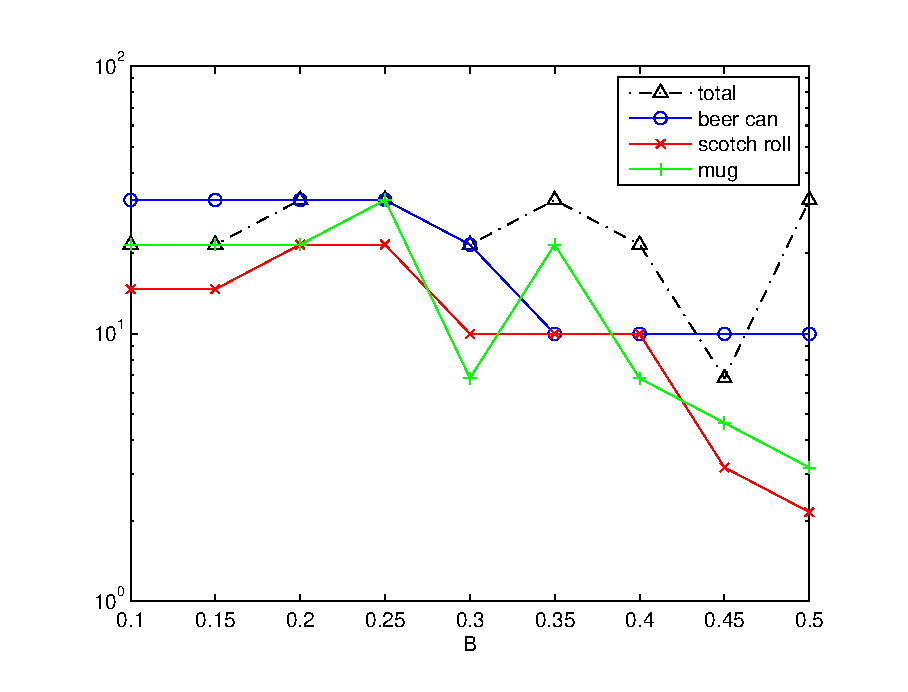
\includegraphics[width=0.5\linewidth]{C_trend.eps}
    \caption{The trend of the hyperparameter $C$ as $B$ is
    increased. $C$ has a definite decreasing trend.}
    \label{fig:C_trend}
  \end{center}
\end{figure}

Let us now focus upon the number of support vectors found by the
SVMs. It turns out that SVMs trained on single objects have roughly
the same number of support vectors as the one trained on the overall
sequence (figures show about $1\%$ more in the first case). This means
that the single-object problems are computationally as hard as the
overall one, but, as we have seen, they are more precise.

Summing up, we can say that if the problem is split into subproblems,
each one regarding a single object, performances are better and the
total computational complexity of the solution remains roughly the
same. This answers the second question.
